
\section{Architecture}
\label{sec:architecture}

Our architecture unifies visual perception and language understanding into a single transformer backbone $f_\theta$, deviating from the standard encoder-decoder pipeline. We process raw pixel patches and text tokens using the same set of weights, allowing for deep, early fusion where the same parameters train jointly across modalities. Clearly however, applying pure language modeling for dense perception tasks (\eg, generating polygon coordinates token-by-token) is computationally expensive. To resolve this, we adopt a hybrid approach: the backbone autoregressively predicts special object tokens (\eg, \texttt{<seg>}), which then act as queries for lightweight, specialized head. This design preserves the simple interface of a language model while enabling the efficient, parallel generation of dense binary masks.


\subsection{Overview}



\noindent We formulate dense perception as a conditional generation task. Given an image $I \in \mathbb{R}^{H \times W \times 3}$ and a text prompt $\mathcal{P} = \{t_1, \dots, t_L\}$, the model must predict a set of $K$ objects $\{O_k\}_{k=1}^K$. Each object is defined by a tuple $O_k = (c_k, s_k, m_k)$ representing its center coordinates, size, and binary segmentation mask. To solve this, we serialize the output into a structured sequence, imposing a ``Chain-of-Perception'' order: $c_k \rightarrow s_k \rightarrow m_k$. This coarse-to-fine curriculum stabilizes training by forcing the model to resolve spatial ambiguity before committing to pixel-level details. The resulting sequence format is \texttt{[Image] [Text] <coord> <size> <seg> $\cdots$ <eos>}, as illustrated in Figure \ref{fig:arch} and \ref{fig:pseudocode}.


\noindent \textbf{Input Representation:} To process these heterogeneous inputs, we flatten the image into $N$ patches and project them into visual embeddings $V \in \mathbb{R}^{N \times d}$. Similarly, the text prompt is mapped to $L$ text embeddings $T \in \mathbb{R}^{L \times d}$. The unified sequence $X \in \mathbb{R}^{S \times d}$ is formed by concatenating these with the task tokens for the $K$ objects, where $S = N + L + 3K$ is the total sequence length and $d$ is the hidden dimension:
\begin{equation}
X = [\underbrace{v_1, \dots, v_N}_{\text{Visual Embeddings}}, \underbrace{t_1, \dots, t_L}_{\text{Text Embeddings}}, \underbrace{e_{\texttt{<coord>}}, e_{\texttt{<size>}}, e_{\texttt{<seg>}}, \dots}_{\text{Task Embeddings}}]
\end{equation}

\noindent The model processes this sequence autoregressively. The backbone $f_\theta$ is a standard dense Transformer with $L$ layers. Processing this sequence requires a specialized attention strategy. Standard causal masking is suboptimal for visual data, as image patches are inherently 2D thus benefit from bidirectional context. We therefore employ a hybrid masking strategy: image tokens attend to all other image tokens (bidirectional), while text and task tokens attend to all image tokens but only to preceding text/task tokens (causal). This allows a single set of weights to act simultaneously as a bidirectional vision encoder and an autoregressive language decoder. Unlike Prefix-LM masking \citep{Beyer2024PaliGemmaAV}, we do not allow prefix text tokens to attend to each other bidirectionally.

\subsection{Specialized Heads}\label{sec:heads}
\begin{wrapfigure}{r}{0.5\textwidth}
  \centering
  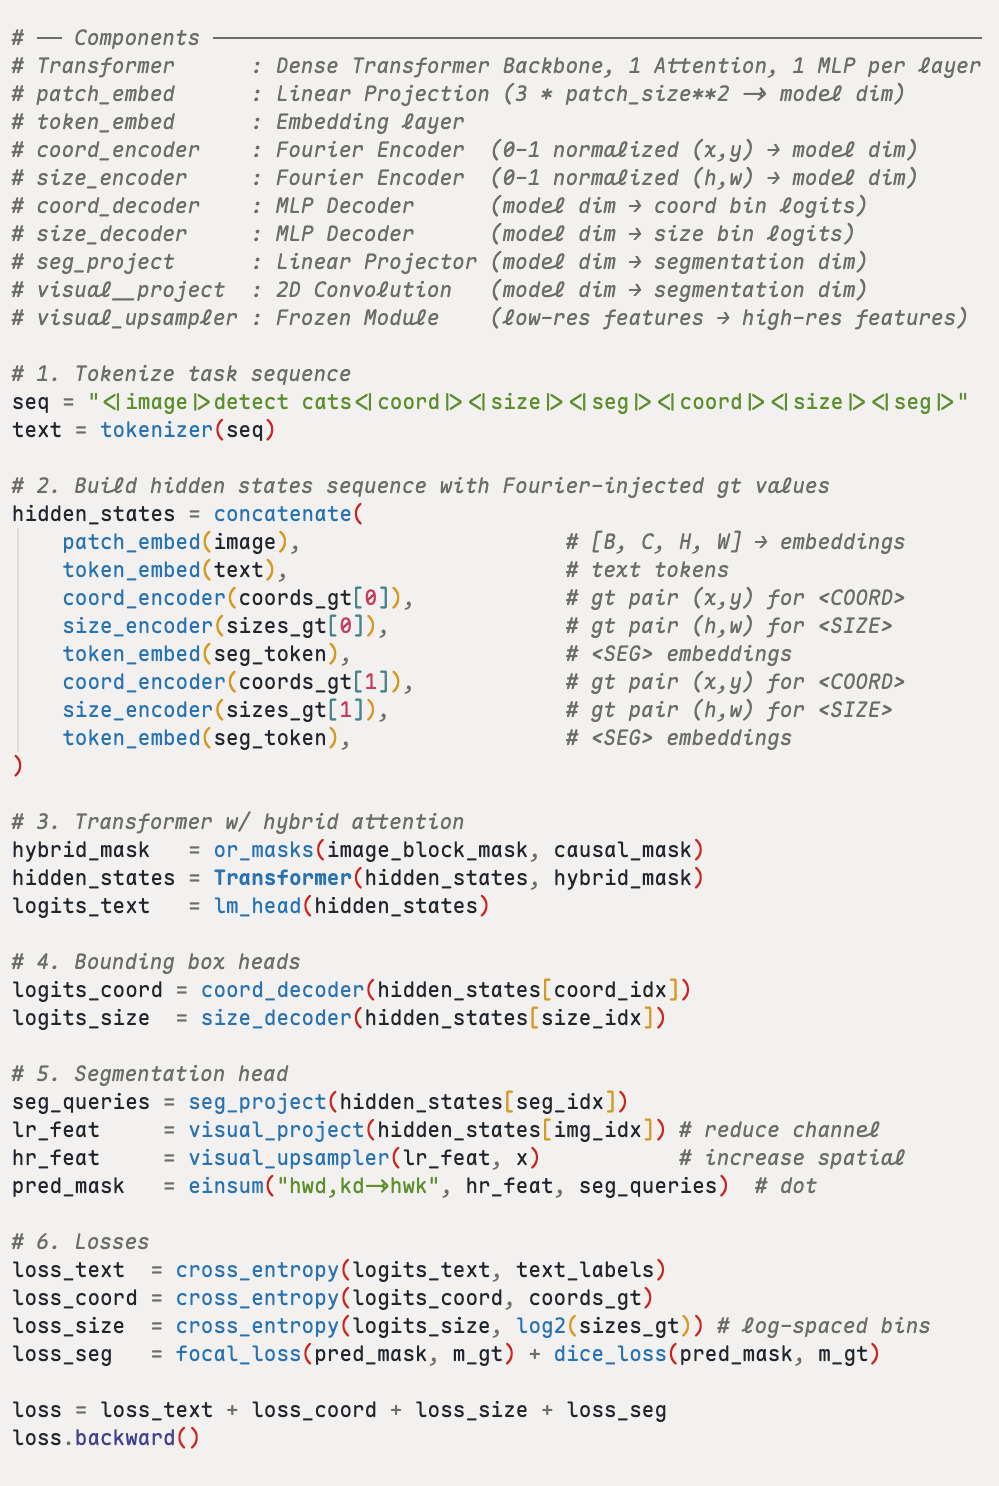
\includegraphics[width=0.5\textwidth]{figures/pseudocode3.png}
  \caption{Training forward pass.}
  \label{fig:pseudocode}
\end{wrapfigure}
While keeping a single Transformer backbone to maximize interaction between tokens of all modalities, we employ specialized encoders and decoders to inject extra inductive biases for spatial task at the input and output layers.


\noindent \textbf{Coordinate \& Size Encoders using Fourier Features:} Standard tokenization of coordinates (\eg, 1000 bins) suffers from limited precision and \textit{spectral bias}, the tendency of neural networks to prioritize learning low-frequency functions, resulting in imprecise spatial grounding.  To overcome this, we adopt a Fourier Feature mapping strategy \citep{FourierFeat}.  We map input coordinates $\mathbf{c} \in [0,1]^2$ to a higher-dimensional feature space using a random gaussian matrix $\mathbf{B} \in \mathbb{R}^{d/2 \times 2}$:
\begin{equation}
\gamma(\mathbf{c}) = [\cos(2\pi \mathbf{B}\mathbf{c}), \sin(2\pi \mathbf{B}\mathbf{c})]
\end{equation}
This projection transforms the coordinate learning problem from a low-dimensional regression (which MLPs struggle with) into a high-dimensional pattern matching task over a rich frequency spectrum. The scale $\sigma$ (set to 10.0) controls the bandwidth of the kernel, tuning the model's sensitivity to fine-grained spatial details. These continuous embeddings are then linearly projected to the transformer dimension and injected directly into the input stream, replacing the static \texttt{<coord>} token. For decoding, we use a simple MLP to project the hidden state into $2 \times N_{bins}$ logits. \textit{Motivation:} predicting coordinates and size \textit{before} segmentation acts as a strong conditioning signal. It forces the model to explicitly resolve instance ambiguity (\eg, "which cat?") and spatial extent. This offloads the localization from the segmentation head, allowing the subsequent \texttt{<seg>} token to focus purely on fine-grained pixel refinement rather than instance discrimination, eliminating the need for heavy mask encoders.


\noindent \textbf{Segmentation (Upsampling + Dot Product):} Generating a high-resolution mask $m \in \mathbb{R}^{H \times W}$ from a single token is challenging. Standard approaches, such as Mask2Former \citep{cheng2022masked}, require complex Hungarian matching to resolve instance ambiguity. We simplify this by leveraging our unified architecture. Since the \texttt{<seg>} token is generated after the coordinates and size, the model has already resolved the object identity. Furthermore, due to our early fusion, its hidden state $h_{seg}$ has direct access to the global visual context. Thus, we can generate the mask via a simple dot product, without separate mask queries.

\noindent To recover fine-grained spatial details, we employ a content-aware upsampler $\mathcal{U}: (V_{out}, I) \to V^*$ \citep{wimmer2025anyup}. This module formulates upsampling as a cross-attention operation where the query is derived from the high-resolution input image $I \in \mathbb{R}^{H \times W \times 3}$ (to guide boundaries), and the key/value are derived from the backbone's output visual features $V_{out} \in \mathbb{R}^{N \times d}$. This allows the model to "paint" semantic features onto the high-resolution pixel grid, producing an enhanced feature map $V^* \in \mathbb{R}^{H \times W \times d}$. The final mask $\hat{m}$ is generated by computing the dot product between these high-fidelity features and the projected hidden state of the segmentation token $h_{seg}$:
\begin{equation}
\hat{m} = \sigma(V^* \cdot \text{Proj}(h_{seg})^T)
\end{equation}

\noindent This design is simple and intuitive, our approach offloads the "localization" to the dense backbone. Because $h_{seg}$ is generated autoregressively and has access to the full early-fusion context $V_{out}$, it already contains the necessary instance-specific information. Consequently, we do not need a separate query learning stage, Hungarian matching, or point-based sampling strategies. The segmentation task is reduced to a straightforward projection, making the architecture easier to implement and scale. 

\subsection{Important Details}

\noindent Beyond the core backbone and specialized heads, several key architectural decisions are needed for handling dense spatial information effectively. We detail these choices below.

\noindent \textbf{3D Rotary Positional Embeddings (Sequence + Space):} To preserve the spatial structure of the input within the flattened sequence $X$, we inject positional information directly into the attention mechanism. Standard 1D RoPE treats the image as a linear sequence, destroying the 2D grid relationships critical for dense prediction. We instead decompose the head dimension $d_{head}$ into two distinct subspaces: a sequential component and a spatial component.

The first half of the head dimension ($d_{head}/2$) encodes the 1D sequence index $t$ using standard RoPE, capturing the causal order of the text tokens and the relative position of patches in the flattened sequence. The second half ($d_{head}/2$) encodes the 2D grid position $\mathbf{p} = (x, y)$ using \textbf{Golden Gate RoPE (GGRoPE)} \citep{xiong2025ndrope}. Unlike standard Axial RoPE, which restricts attention to orthogonal $x$ and $y$ axes, GGRoPE rotates each dimension pair $j$ based on the projection of the spatial position $\mathbf{p}$ onto a unique direction vector $\mathbf{u}_j$:
\begin{equation}
\theta_j = \omega_j (\mathbf{p} \cdot \mathbf{u}_j)
\end{equation}
where the direction vectors $\{\mathbf{u}_j\}$ are sampled uniformly from the unit circle using the Golden Ratio $\phi$. This mechanism allows the attention heads to attend to relative positions along arbitrary 2D angles, producing isotropic attention maps that are robust to rotation and aspect ratio variations. Furthermore, this spatial rotation is applied sparsely only to valid visual tokens, ensuring computational efficiency and preventing interference with text embeddings does not have spatial coordinates.

\noindent \textbf{Native Resolution Handling:} To avoid distorting aspect ratios and degrading performance on small objects. We process images at their native resolution and aspect ratio (up to a maximum token budget). This introduces high variance in sequence lengths: a $256 \times 256$ image yields $\sim 256$ patches, while a $768 \times 768$ image yields $\sim 2,304$. To handle the resulting variance in token counts efficiently, we employ a scatter-and-pack strategy: we patchify the image and discard all padding tokens \textit{before} the transformer, keeping only the valid visual patches. These variable-length sequences are then packed into a single sequence of fixed length $C_{max}$. We utilize FlexAttention to implement the appropriate masking, ensuring that self-attention is restricted within each image sample's boundaries. This maximizes GPU utilization by processing only valid data, but results in a variable number of images per batch across ranks. We address the resulting optimization instability via a global loss balancing strategy \citep{chaybouti2025amoe}.



